\subsection{Hardware Overview}

Hardware aims to work with the software to help the user track what is in the fridge and how long the door is kept open.
The weight sensor tracks the direction of the object in and out of the Smart-Fridge.
The Hal Switch is aware of when the door is open and closed.
The tasks mentioned before run on the ESP-32 microcontroller by Espressif.


This section will also discuss how each of these works in detail, with a record of their power distribution.


\subsection{Power Distribution [ASH]}

The Smart Fridge consists of microcontrollers, logic boards and various sensors which all need to be powered at the appropriate voltage and possible current draw.
Below is a table with all power requirements.


% Please add the following required packages to your document preamble:
% \usepackage{longtable}
% Note: It may be necessary to compile the document several times to get a multi-page table to line up properly
\small
\begin{longtable}[c]{|l|l|l|}
    \caption{Member Contributions and Goals}
    \label{tab:conrib}\\
    \hline
    Team Member &
      Contributions &
      Aims \\ \hline
    \endfirsthead
    %
    \endhead
    %
    Isaac Baglin - IB &
      \begin{tabular}[c]{@{}l@{}}Design Brief: Overview, SAGE assessment\\ form \\  \\ Project Work: Weight Sensor, Esp Camera\\ Module, Buzzer and Debugging  \\  \\ Final Report: System Overview, Smart\\ Fridge Dependency Table, Smart Fridge\\ MOSCOW Diagram, SWOT Analysis, Client\\ Brief Requirement Checklist, Phase Diagram\\ and Description, Weight Sensor Development,\\ Esp32-Wrover Dec-Board Camera\\ Development, Buzzer Development.\end{tabular} &
      \begin{tabular}[c]{@{}l@{}}My goal for this project was to develop\\ skills in systems engineering. To do this,\\ I put myself on the microprocessor team\\ so that I could plan, design, and integrate\\ subsystems.\end{tabular} \\ \hline
    \begin{tabular}[c]{@{}l@{}}Jamie \\ Gomez - JG\end{tabular} &
      \begin{tabular}[c]{@{}l@{}}Design Brief:  Project Management \\  \\ Project Work: Barcode detection, box design \\  \\ Final Report: Economic benefits, Barcode\\ detection, box design prototype 1\end{tabular} &
      \begin{tabular}[c]{@{}l@{}}My aim for this project was to develop my\\ teamwork skills. This was achieved mainly\\ when working on the box design where, \\ throughout the project, it was necessary\\ to listen to the requirements of each team\\ to design a box that best fitted everyone’s\\ needs. \\  \\ With barcode detection my aim was to find\\ and test suitable algorithms in order to\\ select the best one for this product.\end{tabular} \\ \hline
    \begin{tabular}[c]{@{}l@{}}Hamzah \\ Hasnain - HH\end{tabular} &
      \begin{tabular}[c]{@{}l@{}}Design Brief: Sustainability \\  \\ Project Work: Website Creation,\\ LEDs \\  \\ Final Report: Website, LEDs,\\ Sustainability, Circular Economy\end{tabular} &
      \begin{tabular}[c]{@{}l@{}}My goals for this project were to develop my\\ skills, specifically my skills in software and\\ programming. I took responsibility of creating\\ a website. Since I had not previously created\\ a website, there was a lot to learn. Learn how\\ web applications and hardware are integrated \\ I also wanted to gain experience with\\ programming hardware and understand\\ different methods of achieving a software-\\ hardware solution.\end{tabular} \\ \hline
    \begin{tabular}[c]{@{}l@{}}Ioanna \\ Papanikolaou - IP\end{tabular} &
      \begin{tabular}[c]{@{}l@{}}Design Brief: Technical Outline,Sustainability\\ discussion \\  \\ Project Work: \\ Object detection, character recognition,\\ model training  \\  \\ Final Report: Social, Economic and\\ Environmental impacts discussion, Software\\ Section\end{tabular} &
      \begin{tabular}[c]{@{}l@{}}My goals for this project were to develop my\\ software and team working skills. I was in the\\ software team with the aim of developing a \\ model that would classify the objects, acting\\ as an object recognition system. It was also\\ important for me to improve my teamwork\\ skills especially in software as so far I have\\ been mainly working on my own.\end{tabular} \\ \hline
    Yohan John - YJ &
      \begin{tabular}[c]{@{}l@{}}Design Brief: Technical Outline \\  \\ Project Work:  Architect the firmware code,\\ Hal Sensor Integration, Software – Timer\\ for buzzer feature. Comms between\\ raspberry pi and esp32, Debugging.\\ Designed Prototype 1. Designed and\\ built Prototype2 \\  \\ Final Report:  Hardware Outline, Firmware\\ Code, and Box Design and Build Prototyp2\end{tabular} &
      \begin{tabular}[c]{@{}l@{}}My goals for the group project included\\ developing my skills in both the technical\\ and management side. I wanted to take\\ more responsibility for organising the team\\ and architecting the software for the\\ microcontroller. I also aim to be an active\\ team member and contribute resources\\ when required.\end{tabular} \\ \hline
    \begin{tabular}[c]{@{}l@{}}Alexandre\\ Symeonidis-Herzig - ASH\end{tabular} &
      \begin{tabular}[c]{@{}l@{}}Design Brief: Appendices, Latex Compiling,\\ Revising document.  \\  \\ Project Work: Designed Pi Hat (PCB), Power\\ distribution board, Developed React Native\\ App and Created Supabase DB. \\  \\ Final Report: Tech background, Pi Hat PCB\\ design, Power distribution, Mobile App,\\ Supabase DB, Raspberry Pi Refactor\\ as well as compiling in LaTeX, editing\\ the document and formatting citations.\end{tabular} &
      \begin{tabular}[c]{@{}l@{}}To learn about and integrate all the \\ components for an app, from databases\\ and hosting to UI design and functionality.  \\   \\ Also, to focus on the learning the planning\\ required to get a more complicated project\\ from idea to prototype especially with a\\ larger team.\end{tabular} \\ \hline
    Alfie Walding - AW &
      \begin{tabular}[c]{@{}l@{}}Design Brief: Gantt Chart, Project\\ Management, Compiling and Revising\\ document.  \\  \\ Project Work: Raspberry Pi installation\\ and setup, Raspberry Pi camera setup,\\ Barcode detection development,\\ Raspberry Pi Serial communication,\\ Barcode detection integration, OCR code\\ integration, Product detection integration,\\ Supabase database integration and\\ Raspberry Pi refactoring. \\  \\ Final Report: Introduction, Pi Overview,\\ Pi camera, Pi serial input, Pi integration,\\ Pi refactoring as well as compiling and\\ revising the document.\end{tabular} &
      \begin{tabular}[c]{@{}l@{}}To successfully integrate and combine the \\ character, product, and barcode detection\\ code, onto the Raspberry Pi. The code should\\ function together flawlessly with compatibility\\ issues being fixed and required modules \\ imported. \\  \\ To receive data from the ESP and process it \\ into a format that can be communicated to \\ the database.  \\  \\ To successfully detect barcodes in images so\\ they can be sent to the database. \\  \\ To develop skills and knowledge of the\\ Raspberry Pi and the Linux operating system.\end{tabular} \\ \hline
\end{longtable}

As can be seen on the table above, the RPI and ESP-32 consume most of the power and the total system power draw will be around 17W.
However, we will require two separate voltage rails to power the various components, one at 5V and one at 3.3V.
The initial plan to achieve this was to use the adjustable variants of the LM2596.
Using these we could output voltages in the range of 1.2V to 37V at up to 3A with a typical efficiency of 73% [TI DATA SHEET].
We could then power the Smart Fridge's logic components using a 9V power supply which will feed into the two power regulators.
The schematic for these power supplies can be seen below in Figure [X].
Only one power supply is shown in the schematic, as we would use variable resistors to fine-tune the exact voltage in this prototype.


Our 3.3V power supply would be used to power the ESP-32, which has a maximum power draw of 1.65W meaning we will need to input 2.26W (as 2.26* 73% = 1.65W).
At our input voltage of 9V, we would need a minimum current of 0.25A.
Our 5V power supply would be used to power the remaining components, primarily the Raspberry Pi 3B+.
This has a maximum power draw of 15.0525W or roughly 15W.
Meaning we would need to input 22.55W (as 22.55* 73% = 15W) to the power regulator.
At 9V this means we would need an input current of at least 2.28A.
This means for both our power supplies we would need to provide 2.53A at 9V.
To add a safety margin (and due to power supply availability) we would use a 9V power supply capable of providing up the 3A.



Unfortunately, this initial design was not able to be realized due to LM2596 being unavailable.
Availability of this component was not checked before PCB was designed and ordered; this flaw is further discussed in the PCB section.
Fortunately powering the device via other means was also possible, as both the RPI and ESP32 boards have power regulation built in.
This means we can power the RPI using its Micro USB port and power supply capable of delivering the desired 2.5A and then use the GPIO pins 5V output to power the ESP32.
The ESP32 will create a 3.3V output using its built-in power regulator.
The other components listed in table [] above can then be powered using the logic boards outputs and the webcam will still be powered by the RPI as would have been the case originally.



This method is simpler than our previously proposed solution, however there are two major drawbacks; lower efficiency and lower overall power.
Our initial plan used switch-mode power supplies, which adjusts voltage using high-frequencies switching to achieve a high efficiency, however using the onboard voltage regulator of the RPI will give us much lower efficiencies, ranging from 30% to 60%, as they function as variable resistors and turn excess voltage into heat.
These lower efficiencies pose a few problems, first is that the device will draw more power as all times which goes against sustainability targets and may lower a product's energy efficiency rating.
Furthermore, the extra heat may damage the esp32 board, though this is unlikely at our power range, and may cause the RPI to throttle its clock-speed to prevent it from overheating, reducing performance which may be critical for computer vision tasks.
The other drawback is that the total available power to our system, even before inefficiencies, is reduced from 27W to 15W.
This is still enough power for all our systems, as table [] above lists the maximum desired currents, and the minimum power is much lower.
Reduced overall power could lead to power becoming intermittent especially to the webcam and ESP which are downstream from the PI.
However, the RPI documentation states that this should not be an issue as it can pass through around 5W to its GPIO and USB devices, and in practice we found this to hold true however the lack of margin is undesirable.


Overall, the power management did not go as planned due to, in part, the ongoing semiconductor shortage as well as poor planning on the component acquisition side.
However, we were able to pivot to provide a suitable solution and, given more time to order components or redesigning to use a different IC, could make use of the research that went into the original design.


\subsection{PI HAT [ASH]}

In order to securely connect and hold together the various components that make up the Smart Fridge, we designed a printed circuit board.
Using a PCB reduces the chance of connections coming loose, makes the design more compact and increases sturdiness.
In the case of the Smart Fridge, many of our components already come with their own boards (such as the ESP32 dev board or the RPI board) which is why our PCB is designed is designed more as a “motherboard” to hold and connect all the boards.
As the RPI is the largest component of the Smart Fridge the board will be designed as a RPI “Hat” (Hardware Attached on Top) which is a header board specification designed by the Raspberry Pi foundation [RPI GITHUB].
The specifications primairly consist of mechanical specifications, about size, rounding and screw-holes in the PCB, requirements for the 40-pin header used to attach to the RPI, and inclusion of an EEPROM (read only memory) with data about the HAT.
By following these specifications, we ensure that the PCB will fit atop the Raspberry PI and be recognized as HAT.
Our goals for this PCB were to create a board that can, compactly, fit together our various board and sensors, provide them with power and meet the RPI HAT specification.



The PCB was designed in KiCAD which is an open-source and free EDA (Electronic Design Automation) software suite.
KiCAD was chosen as I had previous experience in the software as well as the desire to ensure that anyone on the team be able to open, read and even edit the files using any computer as the software is readily available.
Furthermore KiCAD has a template for RPI HATs that ensure we achieve the desired specifications.
The first step involved placing all of the required components, which consisted mostly of components for the power distribution and connectors for the ESP and other sensors.
Then the appropriate connections where made, as provided by the Hardware team and the power distribution schematics.
A full schematics diagram can be seen on in the appendix [list section].
After this schematic was created the components all had to be given appropriate footprints and then placed on a board.
This completed design can be seen below in Figure [X].



This PCB was then ordered from JLBPCB and assembly began almost immediately of the available components.
Unfortunately there where some problems, firstly, as mentioned in the Power Distribution section the LM2596 were unavailable in our time frame meaning the full board could not be assembled.
Another problem came with the ESP32, as the exact model we ended up using was not the one communicated during the design of PCB and features different pin spacing than most ESP32s, meaning it was too wide to fit on the board.
Initially a “converter” board was considered to allow our new ESP to fit on the PCB, however due to the other problem a different solution was used.
The PCB was also larger than expected due to an export error when sending the files to the manufacturer.
These issues all compounded to leave us with a design that was not fit for function and was therefor abandoned for another solution, the progress up until this point can be seen in the picture below in figure [X].
The created files for the PCB could however easily be updated for a second version had time allowed.



Instead of the PCB, a perfboard was used.
This board was designed using the schematics created for the PCB, as all the connection remained relevant however the EEPROM and Power Distribution section where omitted due to time constraints and redesign respectively.
This board kept the form factor of being mounted atop the RPI, but due to the dropped EEPROM and dimension change can not be considered a PI HAT.
This solution however still serves the original purpose, and manged to provide much of the desired sturdiness and compactness of the original PCB design.


\subsection{Weight Sensor [IB]}

As mentioned previously, the purpose of the weight sensor is to determine whether an item is being placed into the fridge or taken out.
This can be determined if the weight increases, an item is being added and if the weight decreases, an item must be being removed.
The change in weight value will be assigned a direction variable which is communicated to the pi in order to remove or add an item.
For this process to work, the weight value doesn't need to be accurate, however, it must increase or decrease with a change in weight.

The weight sensor which will be used is the HX711 Load Cell.
A load cell contains strain gauges which convert tension on a beam into an electrical signal.
The HX711 contains an 8cm load cell with the strain gauges already attached.
There is also a A/D convertor to convert the tension signal into a usable digital signal for the esp32 to process.
The HX711 Load Cell was chosen specifically because it has libraries available on the Arduino IDE and is compatible with the Esp-32 board.
Figure 1 shows how the Load Cell, A/D convertor and Esp-32 are connected.

\begin{figure}[H]        
    \centering
    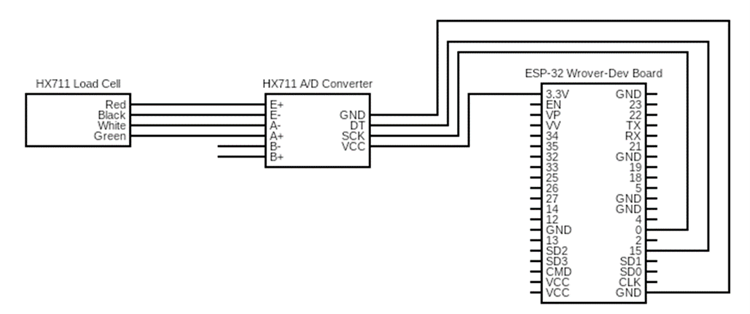
\includegraphics[width=1\textwidth]{Chapter 3/Weight Sensor/LoadCellCircuitDiagram.png}
    \caption{Load Cell Circuit Diagram}
    \label{fig:lccircuit}
\end{figure} 

On the load cell there are 4 holes, 2 on either side which allow us to secure a custom-made platform above and below the load cell.
Because the screws are off cantered, the load cell will be strained when an item is placed on it.
Our load cell is said to support up to 10kg.

\begin{figure}[H]        
    \centering
    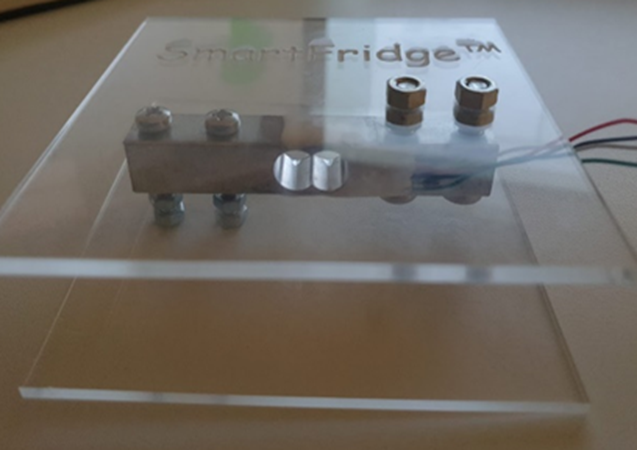
\includegraphics[width=1\textwidth]{Chapter 3/Weight Sensor/WeightSensorPicture.png}
    \caption{Load Cell Prototype}
    \label{fig:lcproto}
\end{figure} 

The HX711 load cell has an Arduino library which contains the necessary functions to calculate the mass in Kg.
Within the setup function, values for calibration\_factor and currentOffset are set.
These helps calibrate the weight to a reasonable value.
Within the loop the function get\_units is used to calculate the mass using the current currentOffset and calibration\_factor values.

\begin{figure}[H]        
    \centering
    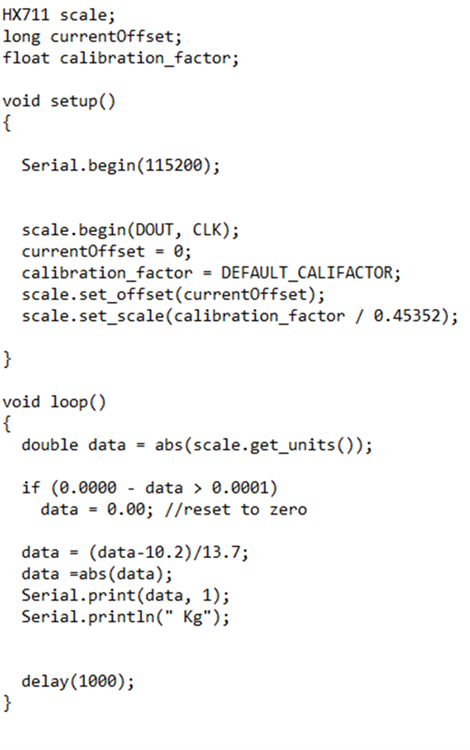
\includegraphics[width=.5\textwidth]{Chapter 3/Weight Sensor/WeightSensorCalibrationCode.png}
    \caption{Load Cell Calibration Code}
    \label{fig:lccode}
\end{figure} 

Often when nothing is placed on the load cell a negative mass is displayed due to an upward force from the table acting in opposition to the weight of the load cell.
To avoid this the mass will be set to zero if it goes negative.
Some manual calibrations are required to offset the fact that the weight can be affected by the weight of the platform as well as how tight the screws are.
Once the load cell has been fitted within the smart fridge these offset values will remain constant after resets.

During the earlier weeks of the project, the load cell platform hadn't been created yet and to test the load cell, it was balanced on a pair of books.
This meant that the strain gauge wasn't being strained correctly as the items were being placed directly on top of it rather than on the correct platform.
This meant that the values were incorrect and couldn't be calibrated correctly.
This resulted in many hours being wasted trying to figure out if something wasn't connected properly or trying to produce elaborate Arduino functions to automatically calibrate the load cell upon the program initializing.

Once a test platform was produced in week 7 using scrap pieces of acrylic, the load cell was able to be calibrated correctly and output accurate results.
An issue which occurred during testing was that the value of the mass continuously fluctuated around its true value.
This was not ideal as the main reason for the weight sensor was to detect changes in weight.
To solve this problem, the mass converted to Kg and given only 1 decimal place.
This meant that the output value didn't fluctuate at all because it output to the nearest 100g.
The trade-off is that the item placed in the fridge must exceed 100g for the weight sensor to detect a difference.
Almost all fridge items are above 100g therefore this wasn't an issue.

\begin{figure}[H]        
    \centering
    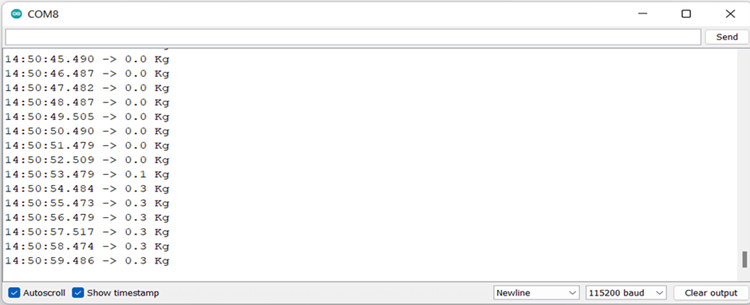
\includegraphics[width=1\textwidth]{Chapter 3/Weight Sensor/LoadCellTestTerminal.png}
    \caption{Load Cell Terminal}
    \label{fig:lcterminal}
\end{figure} 

To test the load cell, it was connected to a terminal and the weight values were printed in the serial monitor.
As expected, when nothing was placed on the load cell, the value was 0kg.
When a 270g weight was placed on the sensor the output value was rounded to 0.3kg whereas a 100g weight output 0.1Kg.
When both items were placed on the senor the combined weight was correctly 0.4kg.

\begin{figure}[H]        
    \centering
    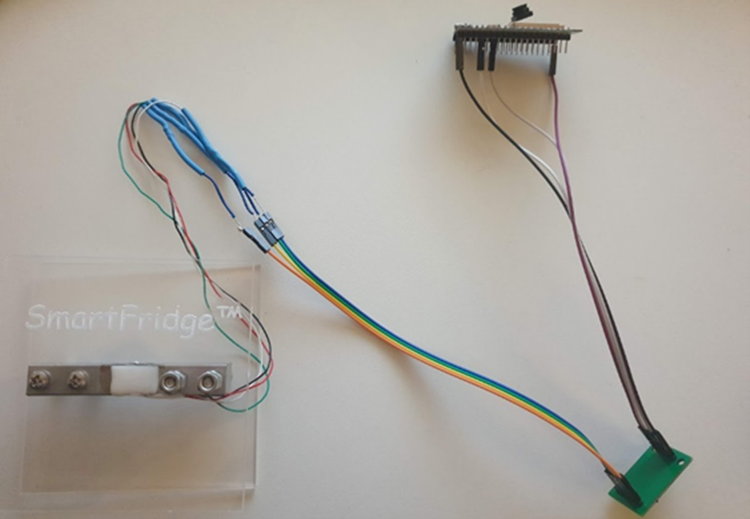
\includegraphics[width=1\textwidth]{Chapter 3/Weight Sensor/WeightSensorWiredImage.png}
    \caption{Load Cell Fully Wired}
    \label{fig:lcwired}
\end{figure} 

It was found that the mass value takes about 2 seconds to stabilise therefore when the code is added to the repository, there should be a 2 second delay between measurements.
When the code was added to the repository, the code in the loop was put in a function which gets the weight of the sensor when called and the setup function was put in a function to setup the sensor.
This meant the entire operation of the weight sensor could be controlled with 2 function calls.

\subsection{ESP-32 Wrover Dev-Board Camera [IB]}

To scan the item, a camera must be placed within the door to detect incoming and outcoming items.
One of the main reasons the Esp-32 Wrover Dev-Board was chosen was due to it having a camera connected directly to a microprocessor.
Typically, external esp cameras require over a dozen connections to the microprocessor.
This would greatly increase the complexity of the build and could result in extensive soldering which could lead to errors such as poor connections and information loss.
Also, by having the camera connected directly to the board, there is now more pins available to connect the other components to.
The board contains 2 cores, this allows the processor to run multiple tasks at the same time instead of unnecessarily waiting.

There is an Arduino IDE library called 'esp\_camera.h' which contains functions that control the operation of the camera.

\begin{figure}[H]        
    \centering
    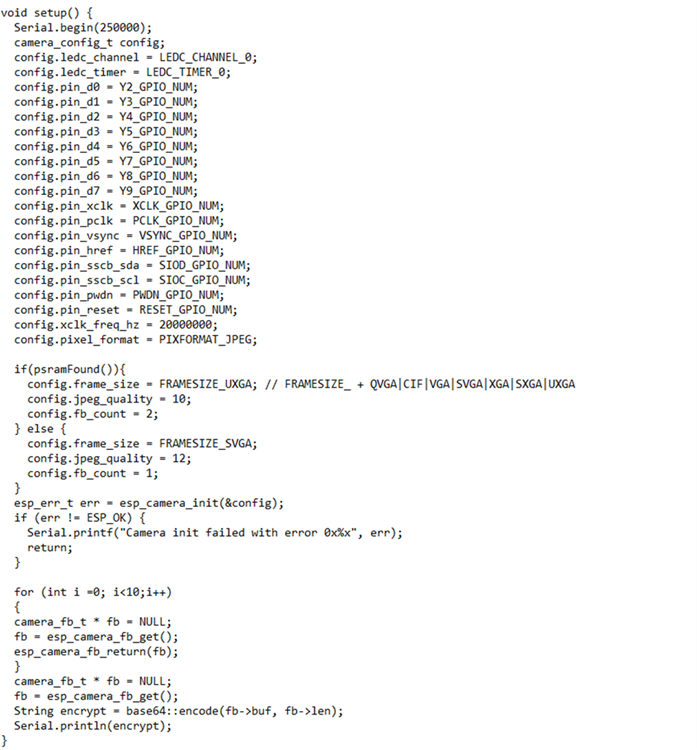
\includegraphics[width=0.75\textwidth]{Chapter 3/ESP-32 Wrover Dev Board/ESP32Camera.png}
    \caption{ESP Camera Code}
    \label{fig:espcamcode}
\end{figure} 

A config object needs to be created so that the pins can be assigned.
Given that the camera is connected directly to the board, the pin configuration is defined on the board's datasheet.
The quality of the jpeg is determined by the member variable jpeg\_quality.
It is crucial that the jpeg quality is maximised so that a clear image is sent to the OpenCV program to read the barcode.
To take a photo the buffer variable fb must be set to null.
The function esp\_camera\_fb\_get() is used to take the photo and store in fb.

The image will be packaged with the weight and the ON/Off state and sent via serial to the raspberry pi to be processed.
A major issue that was faced was that jpeg images can't be sent over the serial to the raspberry pi, only Integers, strings etc.
To fix this issue, a base64 encoder was used to encode the image as a base64 string.
This string can be sent via the serial and decoded back into a jpeg in the raspberry pi.
A base 64 string is around 170 thousand characters and can be captured and sent via serial in around 1 second.
Considering the weight sensor takes a similar amount of time, threading will be easier as they can both start and finish their tasks simultaneously and be sent together without excess delay.

\begin{figure}[H]        
    \centering
    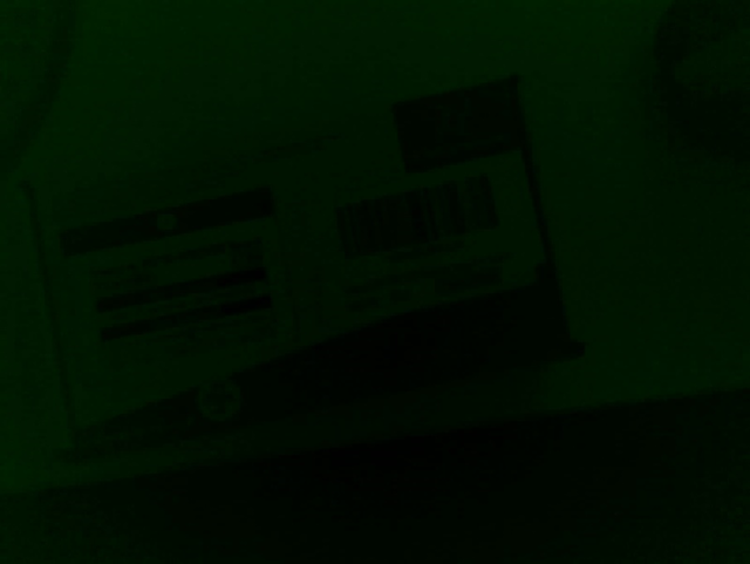
\includegraphics[width=1\textwidth]{Chapter 3/ESP-32 Wrover Dev Board/ESP32Picture.png}
    \caption{First Picture from ESP Camera}
    \label{fig:espcamfp}
\end{figure} 

When the code was uploaded to the board, the program would crash due to there being no more room for the buffer.
At first it was believed that this error was because the size of the buffer was too big.
To reduce the file size, the jpeg quality was reduced by making the variable jpeg\_quality smaller.
Even after this change, the same error occurred.
It was then found that the issue wasn't the size of the buffer but the fact that it wasn't reset after the photo was taken.
This was causing the memory to leak.
The function esp\_camera\_fb\_return(fb) was used after each photo to return the buffer and the jpeg quality was changed back to the maximum value.

Once this error had been fixed a 170 thousand character string was printed to the serial whenever a photo was taken.
The next problem faced was that the photo which was taken was very dark and had a green filtered look.
This can be seen in figure 10.

At first it was thought that this issue was due to data loss by encoding and decoding an image in base64 however it was found that when using base64 on random jpeg images from the internet, this green distortion wasn't found.
Typically, this camera module is used to stream 30fps video to a server, therefore it goes against the original function of the module to take isolated photos.
After extensive research it was found that multiple images need to be taken to “warm up” the camera before saving the final photo.
To do this, a ten iteration for loop was added before the final capture to take and delete “warm up” photos.
This process effectively simulates the first 333ms of a video recording as the camera begins operation.
After integrating this into the code a photo was output which no longer had a green look to it.

\begin{figure}[H]        
    \centering
    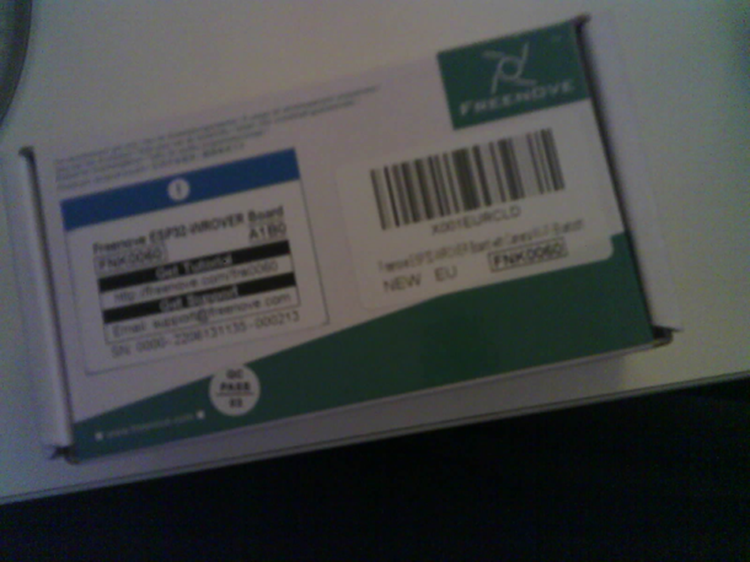
\includegraphics[width=1\textwidth]{Chapter 3/ESP-32 Wrover Dev Board/ESP32BetterPicture.png}
    \caption{Better Picture from ESP CAM}
    \label{fig:espcambetterpic}
\end{figure} 

The number of warm up photos taken was altered to identify the effect and it was found that 10 is the number where the quality doesn't get noticeably any better.

The base64 image was sent to the raspberry pi to use the OpenCV code to detect the barcode on the image.
Unfortunately, the code was unable to detect the barcode in the image.
Dozens of images were tested, each with different angles, distances and focuses and in not one example was the program able to detect the barcode.
It was concluded that the camera resolution wasn't high enough to accurately detect the thin lines of the barcodes.
Given that the resolution of the camera was already maximised, there was very little that could be done to improve it.
Lots of time could be spent trying to find the perfect conditions to take the photo however in the final product the camera will be fitted within the fridge therefore there will be no control over things like angle and distance without heavily disrupting the user experience.

With time and the customer in mind, it was decided that the esp camera was no longer going to be used.
Instead, a web camera will be connected directly to the raspberry pi.
This will ensure a high-quality image is sent to the OpenCV program as well as simplify the product by not needing to encode and decode the image across the serial.
When tested, the program was able to accurately detect the barcode.
Given that the rest of the hardware was built around this esp board, it will continue to be used however the camera module will be disconnected.

\subsection{Buzzer [IB]}

Once the fridge door is open, a timer will start.
Once this timer has reached a certain time a buzzer will activate to remind the user to shut the fridge door.
The 85dB Panel Mount Continuous Internal Piezo Buzzer will be used due to its small size and its low price.
The tone of the buzzer is determined by the frequency set via the esp pin.
Two connections are required for this buzzer, a pin connection and ground.

\begin{figure}[H]        
    \centering
    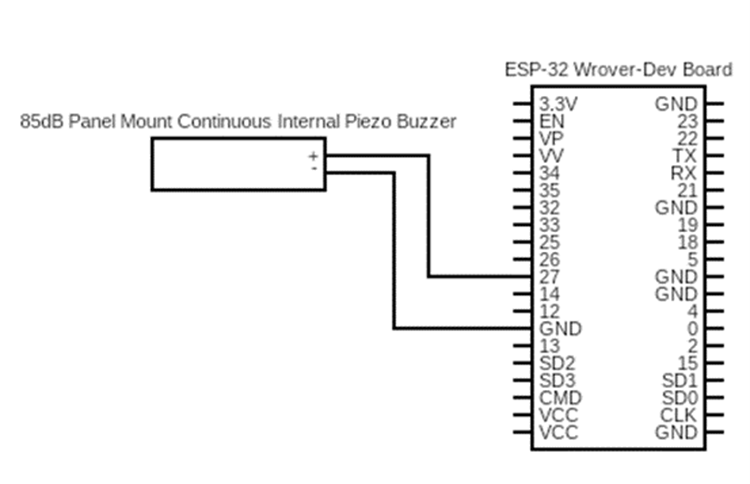
\includegraphics[width=1\textwidth]{Chapter 3/Buzzer/BuzzerCircuitDiagram.png}
    \caption{Buzzer Circuit Diagram}
    \label{fig:buzzcircuit}
\end{figure} 

The tone will be set to 1kHz and sound on and off every second.
Pin 27 is assigned as an output pin and will send 1 kHz signal to the buzzer using the function called 'tone'.
A 1 second delay will keep the buzzer on using the function called 'delay'.
The buzzer will then be turned off using 'noTone'.
A further delay was added to keep the buzzer off for 1 second before the loop begins again.
When tested, the buzzer produced a loud 1kHz alarm that sounded on and off every second.
After some experimenting, it was found that decreasing the frequency and increasing the delay made the buzzer sound less alarming whereas increasing the frequency and decreasing the delay made the sound from the buzzer sound too irritating to listen to and it therefore might harm the user's experience.
The frequency and delays were kept at 1kHz and 1 second.
The code was then wrapped in a function and added to the repository to be called when the fridge door timer runs out.


\subsection{HAL Sensor [YJ]}

Fridges need to know when the door is open or when the door is closed.
There are numerous ways to do this, a mechanical switch or implementing a HAL effect sensor.
Our Product uses the latter.
All fridges use magnets to create a soft close door feature and to hold the door closed.

\begin{figure}[H]        
    \centering
    
\includegraphics[width=1\textwidth]{Logo.png}
    \caption{Place Holder: Magnet Pic}
    \label{fig:placeholder}
\end{figure} 

The Hall effect switch will turn on in the presence of a south magnetic field on its face or a north magnetic field on the opposite side.
It will turn off when the magnet is not in range.

\begin{figure}[H]        
    \centering
    
\includegraphics[width=1\textwidth]{Logo.png}
    \caption{Place Holder: HAL Code}
    \label{fig:placeholder}
\end{figure} 

We can monitor the sensor readings as shown above, and if there is a change in the state, we know when the door is open or closed.
In our feature, the sensor returns True when the doors are open and False when the doors are closed.

